\documentclass[final,12pt]{elsarticle}

% Load required packages
\usepackage[utf8]{inputenc}
\usepackage[T1]{fontenc}
\usepackage{amsmath}
\usepackage{amsfonts}
\usepackage{amssymb}
\usepackage{graphicx}
\usepackage{lineno}
\usepackage{longtable}
\usepackage{pdflscape}         % For landscape pages
\usepackage{xcolor}            % For custom colors
\usepackage{tikz}             % For creating diagrams and flowcharts
\usetikzlibrary{positioning}  % For relative positioning in TikZ
\usetikzlibrary{shapes.geometric}  % For geometric shapes in TikZ
\usepackage[most]{tcolorbox}  % For creating boxed environments with all libraries
\usepackage{hyperref}  % For clickable links and citations

% Fix for elsarticle page breaking issues
\raggedbottom
\setlength{\textfloatsep}{5pt plus 1pt minus 2pt}
\setlength{\floatsep}{5pt plus 1pt minus 2pt}
\setlength{\intextsep}{5pt plus 1pt minus 2pt}

% Define custom prompt environment using tcolorbox
\definecolor{promptbg}{RGB}{250,250,250}
\definecolor{promptframe}{RGB}{200,200,200}
\newtcolorbox{prompt}{
    breakable,
    colback=promptbg,
    colframe=promptframe,
    boxrule=1pt,
    left=1em,
    right=1em,
    top=0.5em,
    bottom=0.5em,
    arc=0pt,
    boxsep=0pt,
    before skip=0.5em,
    after skip=0.5em
}

% Journal name (replace with actual journal name)
\journal{Environmental Modelling \& Software}

% Highlights section
\begin{document}

\begin{highlights}
\item AI framework automates species grouping and diet matrix creation with >99.7\% consistency
\item Framework correctly identifies 85\% of trophic interactions with high ecological accuracy
\item LLM-driven synthesis integrates global databases with unstructured local knowledge
\item Reduces ecosystem model development time from months to hours with 80\% diet accuracy
\end{highlights}

\title{AI-Driven Knowledge Synthesis for Food Web Parameterisation}

% Author information in elsarticle format
\author[1,2]{Scott Spillias\corref{cor1}}
\author[1,2]{Elizabeth A. Fulton}
\author[2,3,4]{Fabio Boschetti}
\author[1]{Cathy Bulman}
\author[3]{Joanna Strzelecki}
\author[1,2]{Rowan Trebilco}

\cortext[cor1]{Corresponding author: scott.spillias@csiro.au}

\address[1]{CSIRO Environment, Hobart, Australia}
\address[2]{Centre for Marine Socio-Ecology, University of Tasmania, Hobart, Australia}
\address[3]{CSIRO Environment, IOMRC Crawley, Australia}
\address[4]{Oceans Institute, The University of Western Australia, Crawley, WA}

% Keywords
\begin{keyword}
Artificial Intelligence \sep Ecological Modelling \sep Ecopath with Ecosim \sep Diet Interaction \sep Large Language Models
\end{keyword}

\begin{abstract}
This study introduces a novel Large Language Model (LLM) driven framework for automated species grouping and food web construction for ecosystem models, addressing a bottleneck in model development. The framework retrieves marine species lists from an area, uses LLMs to classify them into functional groups; and synthesizes trophic interactions from diverse data sources including global biodiversity databases and unstructured user-provided text. Evaluation across four Australian marine regions demonstrates high reproducibility in species grouping (>99.7\% consistency) and food web construction, with 51-59\% of predator-prey interactions showing consistent proportions across runs. Validation against expert-derived food webs for the Great Australian Bight reveals strong ecological accuracy, with 92.6\% of assignments being at least partially correct, and correctly identifying 85\% of trophic interactions. The framework estimates interaction strengths within 0.2 of expert values for 80\% of interactions. These findings demonstrate the potential to generate reproducible, plausible food webs while reducing development time to hours.
\end{abstract}

\maketitle

% % Graphical Abstract
% \begin{figure}
% \centering
% 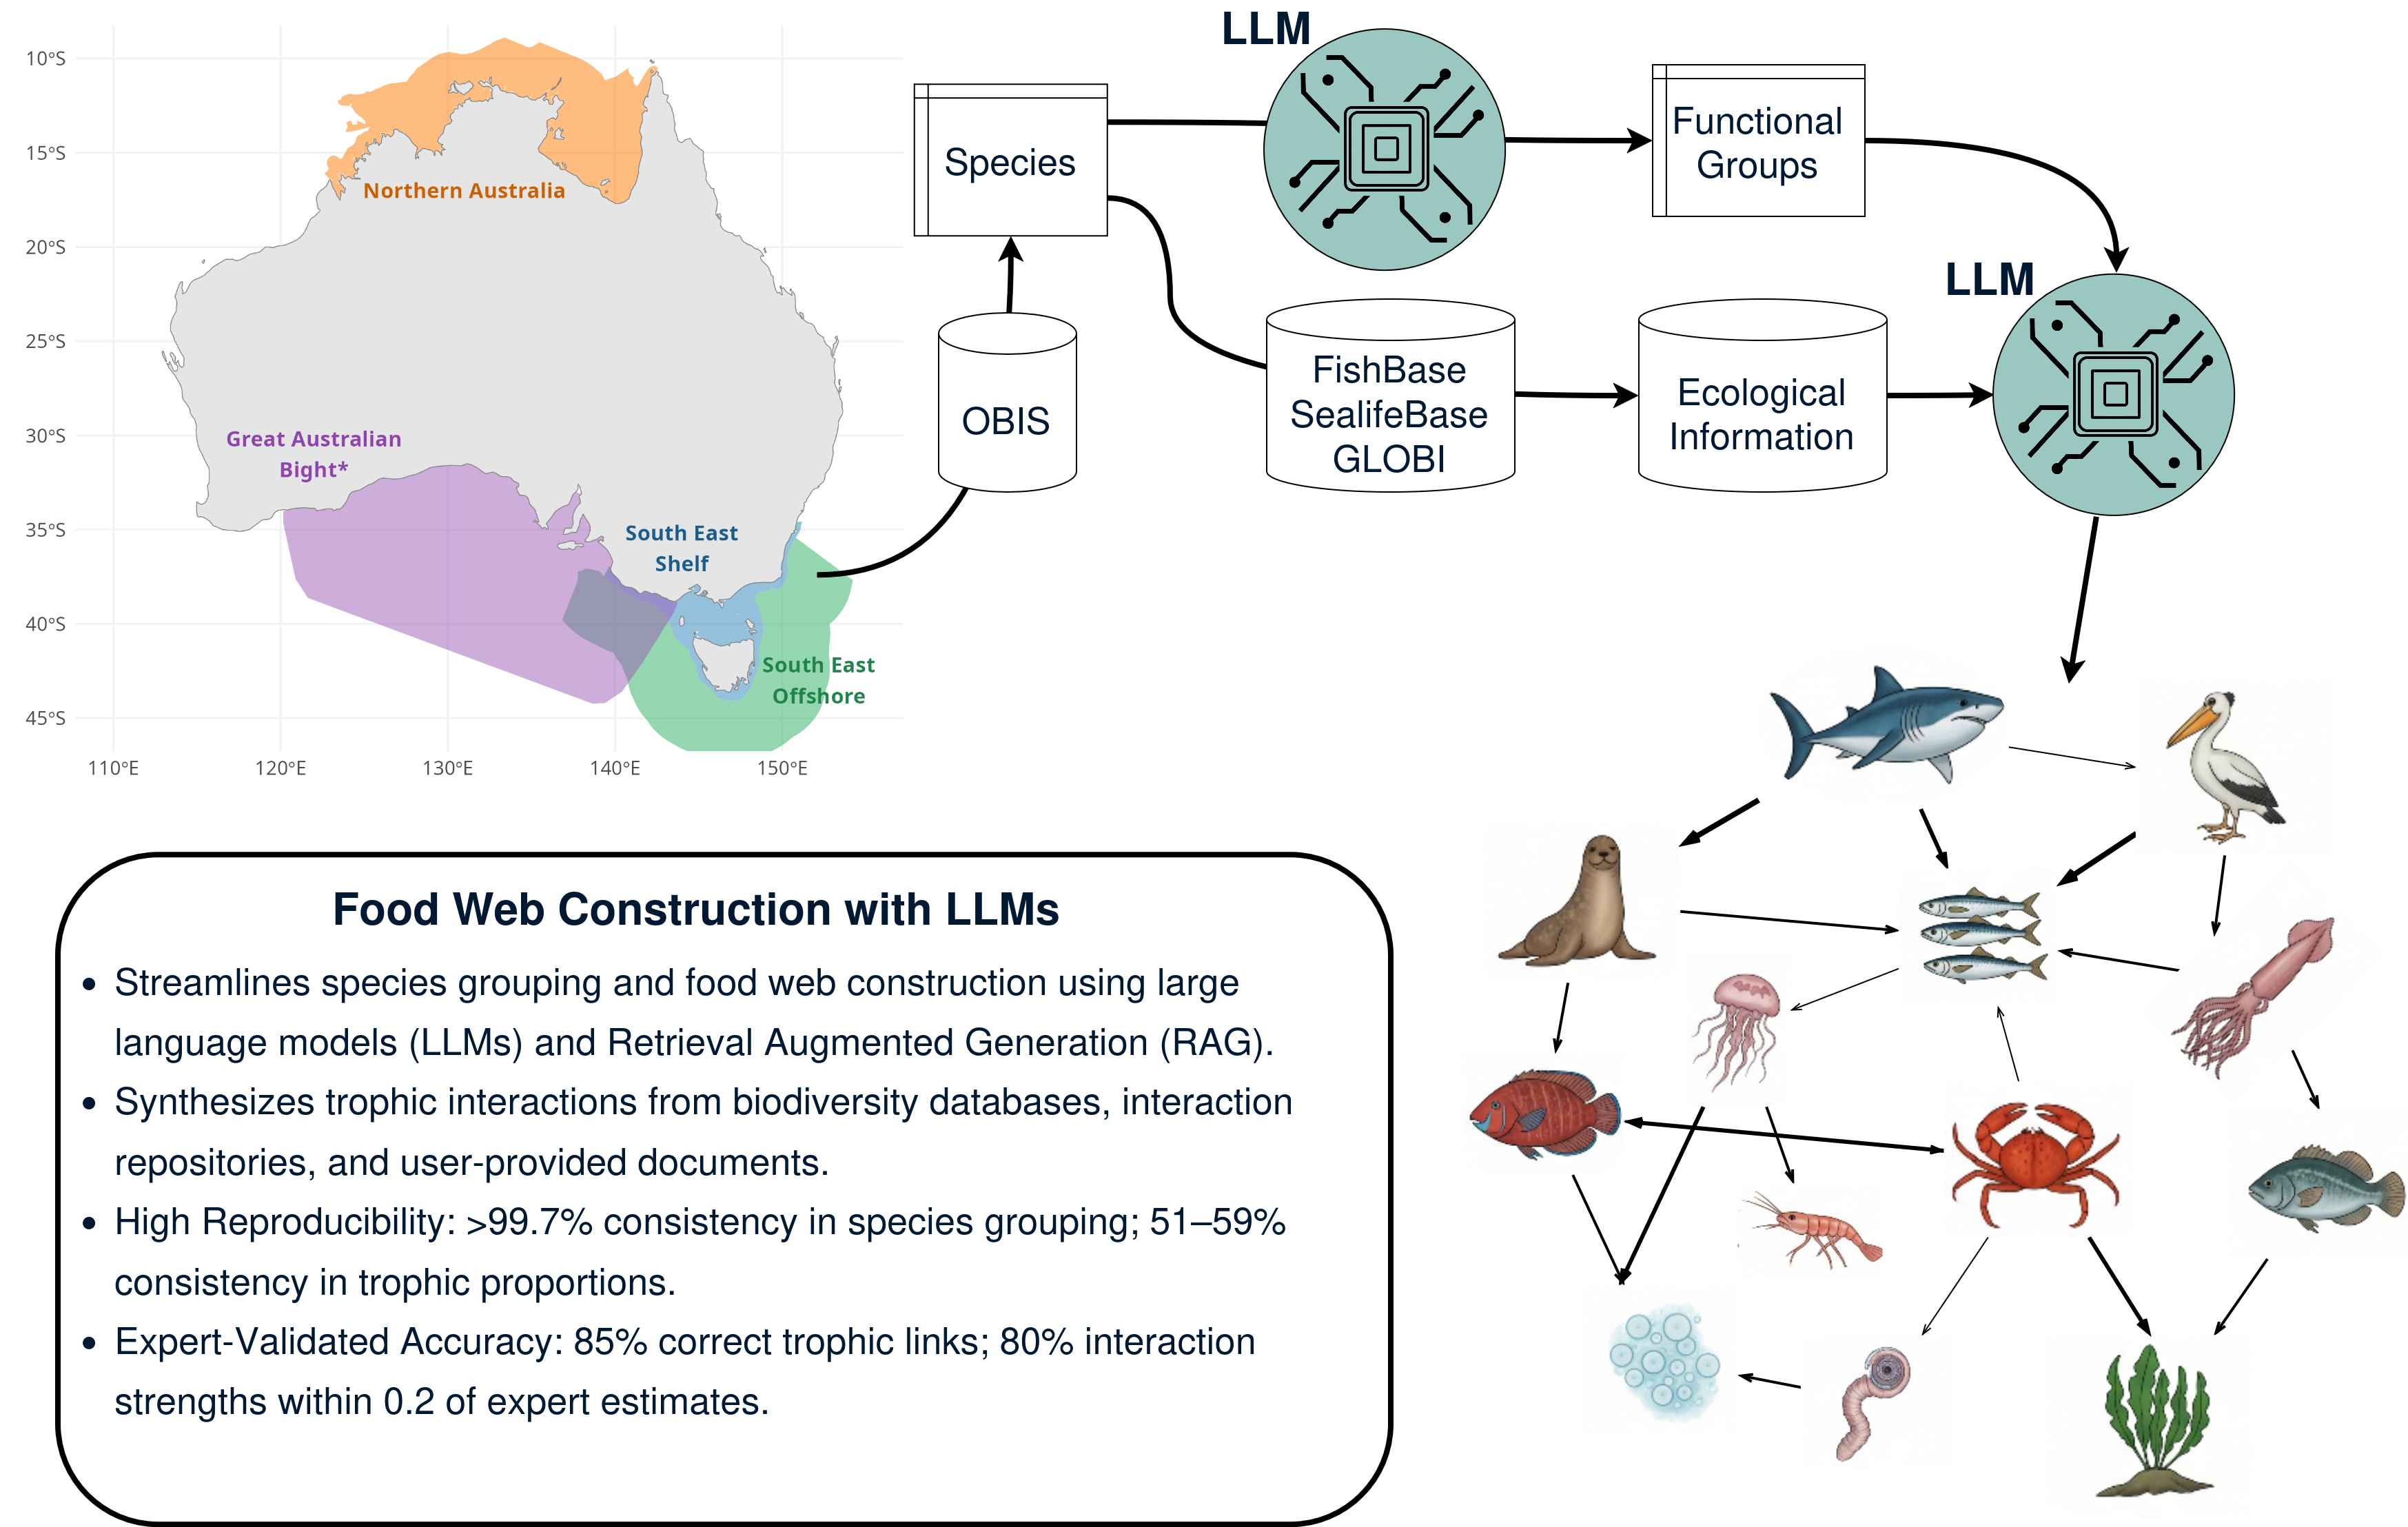
\includegraphics[width=0.8\textwidth]{figures/GraphicalAbstract.png}
% \caption*{Graphical Abstract: AI-Driven Knowledge Synthesis for Food Web Parameterisation}
% \end{figure}

\linenumbers

\input{1_introduction}
\input{2_methods}
\input{3_results}
\input{4_discussion}

\section*{Acknowledgements}
SS was funded by a CSIRO R+ Postdoctoral Fellowship. This project was partially funded by the `Futures of Seafood' project.

\section*{Software Availability}
The complete codebase, including all scripts, configuration files, and analysis tools, is available at https://github.com/s-spillias/AI-EwE-Diets. The validation framework, including reference group definitions and classification rules, is documented in the project repository to ensure reproducibility.

\section*{Author Contributions}
SS: Conceptualization, Methodology, Software, Validation, Formal analysis, Investigation, Resources, Data Curation, Writing - Original Draft, Writing - Review \& Editing, Visualization, Project administration. BF: Validation, Writing - Review \& Editing, Supervision, Funding acquisition. FB: Methodology, Software, Validation, Writing - Review \& Editing, Supervision. CB: Investigation, Data Curation, Validation, Writing - Review \& Editing. JS: Conceptualization, Validation, Investigation, Writing - Review \& Editing. RT: Methodology, Software, Validation, Investigation, Writing - Review \& Editing, Supervision, Funding acquisition.

\section*{Statement on the Use of Generative AI}
Generative AI tools, specifically Claude Sonnet 3.5, were utilized in the preparation of this manuscript to assist with tasks such as language refinement, text structuring, and summarization. All scientific content, data interpretation, and conclusions were independently developed and verified by the authors to ensure accuracy and integrity.

\bibliographystyle{elsarticle-harv}
\bibliography{references}

\clearpage
\input{5_supplement}

\end{document}